\subsection*{Grey Box Sequence Diagram}
\begin{figure}[H]
	\centering
	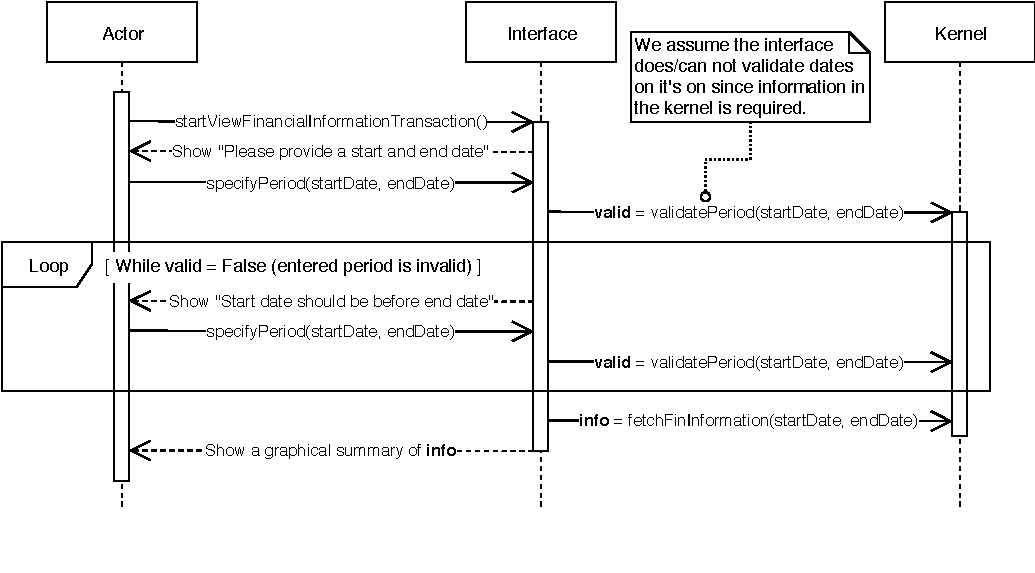
\includegraphics[scale=.9]{uml/SD-gb-finInformation.pdf}
	\caption*{Grey Box diagram for use case C3, made by A}
\end{figure}
The interface in a grey box acts as an intermediate step between the actor and the kernel. User commands are passed to the interface, and it in turn can do some minor operations before delegating it to the kernel.\\For example, in this case, when we receive the starting and ending dates for the period the actor wants to view the financial information of, we need to decide whether this is a valid period first. We `translate' the request ``specifyPeriod(..)'' to the interface into the more generic ``validatePeriod(..)'' which we pass to the kernel to do the computation. We only keep this period if it is a valid period. Otherwise we ask the actor to retry. We then ask the kernel to fetch the finantial information which we show to the actor. We do not state what this information entails in the gray box, because if we later decide there is more financial information that we need to fetch, we only need to update the white box implementation.
\subsection*{White Box Sequence Diagram}
\begin{figure}[H]
	\centering
	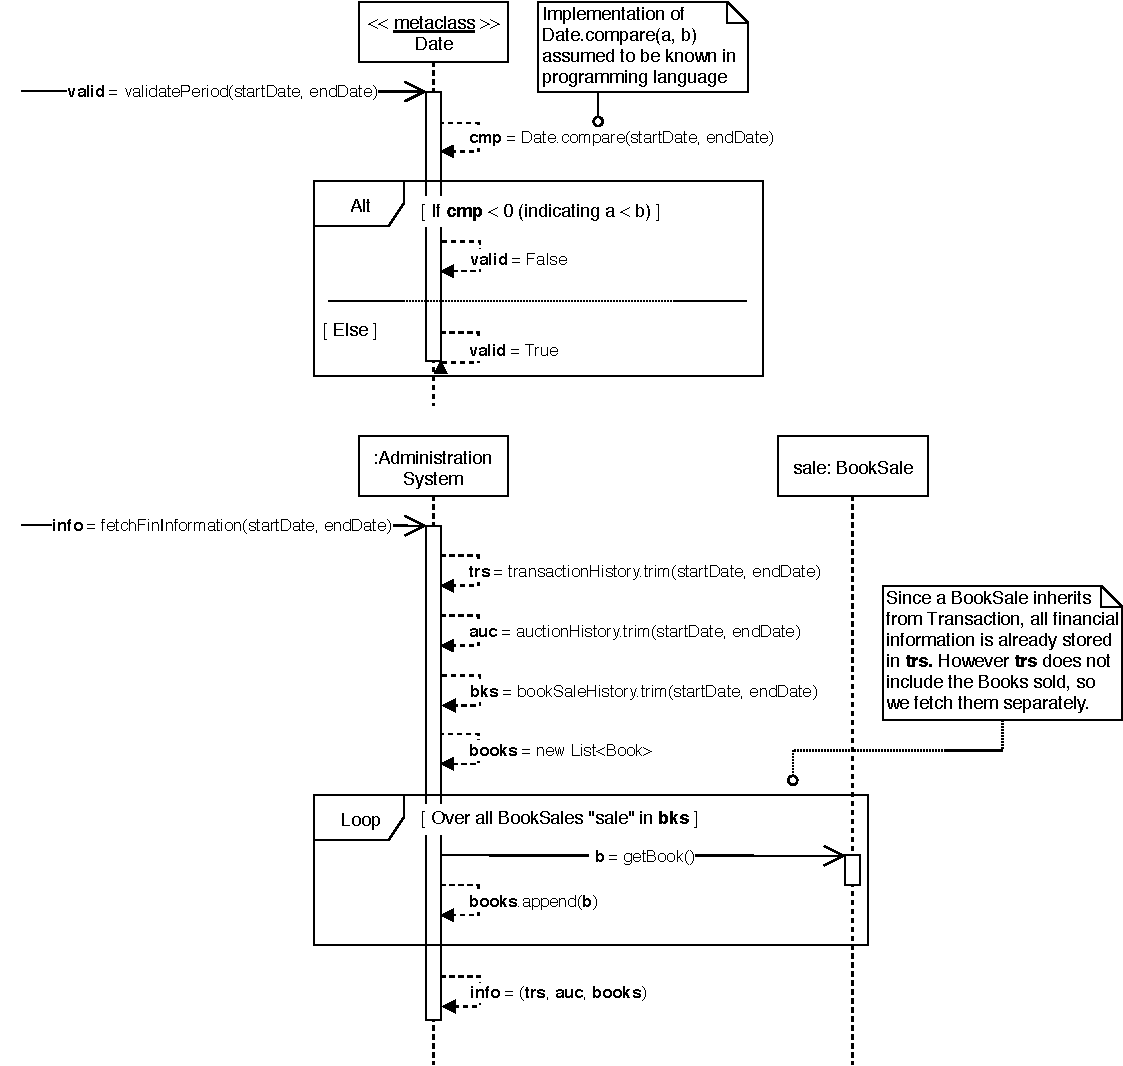
\includegraphics[scale=.70]{uml/SD-wb-finInformation.pdf}
	\caption*{White Box diagram for use case C3, made by A}
\end{figure}
The white box is a high level implementation diagram for all kernel operations. The interface and actor are out of the picture, and everything is viewed from an implementation point of view. We pass all kernel requests to a single class that will decide how to distribute the requests. This is to avoid having to rewrite the top level implementation when we want to change the implementation for something simple and low level.\\As an example, the ``fetchFinInformation()'' function to the user class (found in the class diagram) is being delegated and executed in the AdministrationSystem class. This class in turn collects all information it needs to summarize the financial information and returns it.\\
An exception is the ``validatePeriod(..)'' request, which is delegated to the static class Date. Since it is highly unlikely that we modify this request internally, we can avoid passing this simple request through the User class.